\documentclass[conference]{IEEEtran}

\usepackage{cite}
\usepackage{pslatex} % -- times instead of computer modern, especially for the plain article class
\usepackage[colorlinks=false,bookmarks=false]{hyperref}
\usepackage{booktabs}
\usepackage{graphicx}
\usepackage{xcolor}
\usepackage{multirow}
\usepackage{comment}
%\usepackage{flushend} % even out the last page, but use only at the end when there is a bibliography

\newcommand{\code}[1]{{\small{\texttt{#1}}}}

% fatter TT font
\renewcommand*\ttdefault{txtt}
% another TT, suggested by Alex
% \usepackage{inconsolata}
% \usepackage[T1]{fontenc} % needed as well?

\usepackage{listings}

%\newcommand{\todo}[1]{{\emph{TODO: #1}}}
\newcommand{\todo}[1]{{\color{olive} TODO: #1}}
\newcommand{\martin}[1]{{\color{blue} Martin: #1}}
\newcommand{\andrew}[1]{{\color{red} Andrew: #1}}
\newcommand{\rewrite}[1]{{\color{red} rewrite: #1}}

% uncomment following for final submission
%\renewcommand{\todo}[1]{}
%\renewcommand{\martin}[1]{}


%%Uncomment the following when you want to add copyright notice and not use any space	 (IEEE only)
%\usepackage[absolute]{textpos}
%% Set unit to be pagewidth and height, and increase inner margin of box
%\setlength{\TPHorizModule}{\paperwidth}\setlength{\TPVertModule}{\paperheight}
%\TPMargin{5pt}
%% Define \copyrightstatement command for easier use
%\newcommand{\copyrightstatement}{
%	\begin{textblock}{0.85}(0.072,0.93)    % Tweak here: {box width}(leftposition, rightposition)
%		\noindent
%		\normalsize
%		???-?-?-???-?/??/\$31.00~\copyright20?? IEEE % Put here your copyright
%	\end{textblock}
%}

\begin{document}


%\title{Towards Verification of Digital Circuits with\\
%SystemVerilog/UVM and Chisel/Scala}

\title{Open-Source Fuzzing-based Verification\\ with Chisel and Scala}

\author{


\IEEEauthorblockN{Andrew Dobis, Tjark Petersen, Martin Schoeberl}
\IEEEauthorblockA{\textit{Department of Applied Mathematics and Computer Science} \\
\textit{Technical University of Denmark}\\
Lyngby, Denmark \\
andrew.dobis@alumni.epfl.ch, s186083@student.dtu.dk, masca@dtu.dk}
}


\maketitle \thispagestyle{empty}

\begin{abstract}

Verification of Digital Systems ...

\end{abstract}

\begin{IEEEkeywords}
digital design, verification, fuzzing
\end{IEEEkeywords}

\martin{We aim for \url{https://woset-workshop.github.io/WOSET2020.html}}

\section{TODO}

Ref our last WOSET paper

\todo{Rewrite all what is left over now, as this is a copy of the last WOSET paper and from the verify paper}


\section{Introduction}
\label{sec:intro}

In recent years, we have seen an increase in the demands for high performance computing systems.  
This comes with an increase in the need for domain-specific hardware accelerators.  
Designing these is time-consuming and error prone, which is why researchers have been focusing on increasing the efficiency of Hardware Verification tools to fight this added time constraint.
This has lead to the introduction of verifications methods, such as constrained random verification and functional coverage~\cite{verify:chisel:2020, dobis2021opensource}, into high level hardware construction languages, like the Scala-embedded language Chisel~\cite{chisel:dac2012, chisel:book} .
These tools, inspired by the more hardware-centric approach given in SystemVerilog and UVM, enable basic verification, where the user has to handle the writing of all tests by hand.
To improve the efficiency of these tools, we propose a form of dynamic verification, based on coverage-driven mutation-based fuzzing techniques found in the Software world.
This allows for optimal fuzzing for RTL designs using functional coverage as a metric to drive the fuzzing.

This paper describes a research project that aims to develop an optimal functional coverage-driven mutation-based fuzzing tool to test RTL circuits.
We the plan on building upon this tool to enable constrained random program generation allowing for fuzzing to be used to test processors.

This paper is organized in six sections: % The following section presents related work.
Section~\ref{sec:related}  Presents related work.
Section~\ref{sec:tools} describes the open-source tools that we use in our project.
Section~\ref{xxx} presents our open-source fuzzing library, which is part of ChiselVerify.
Section~\ref{sec:eval} evaluates our approach with a small design example written in Chisel, VHDL,
and Verilog.
Section~\ref{sec:conclusion} concludes.


%\rewrite{Recent advances with SystemVerilog and Chisel \cite{chisel:dac2012, chisel:book} have brought object-oriented programming
%into the digital design and verification process. SystemVerilog, an extension of Verilog, adds object-oriented concepts for the non synthesizable verification code.
%Chisel is a ``Hardware Construction Language'', embedded in Scala, to describe digital circuits.
%Circuits described in Chisel can be tested and verified with a Chisel testing framework and Scala tests.
%Scala/Chisel brings object-oriented and functional programming into the world of
%digital design.
%
%
%This paper describes a research project that aims to build a testing framework in Scala
%that takes the best methods from the Universal Verification Methodology (UVM) and
%decades of experience in software testing.
%Furthermore, we aim to build on open-source projects only. Therefore, our
%work is open-source as well.
%
%The main contribution of this paper is
%
%This paper is organized in six sections: % The following section presents related work.
%Section~\ref{sec:related}  Presents related work.
%Section~\ref{sec:tools} describes the open-source tools that we use in our project.
%Section~\ref{xxx} presents our open-source fuzzing library, which is part of ChiselVerify.
%Section~\ref{sec:eval} evaluates our approach with a small design example written in Chisel, VHDL,
%and Verilog.
%Section~\ref{sec:conclusion} concludes.}
%


\section{Related Work}
\label{sec:related}
We will now present work related to current developments in hardware verification and fuzzing for RTL circuits.

\martin{What does SV and UVM bring on the table related to fuzzing? Someone must have tried it.}
\andrew{Fuzzing is a very software thing to do, it's only been noticed by verification engineers in recent years, the only "completed" work I've found on fuzzing for hardware is Kevin's stuff. Everything else is very conceptual and not complete.}

The Universal Verification Methodology (UVM) is a methodology for testing and verifying of digital circuits.
UVM is implemented as a SystemVerilog library and utilizes the fact that SystemVerilog uses object-oriented programming when designing testbenches.
Using object-oriented patterns such as inheritance and polymorphism, the verification engineer can design generic components that can be extended and modified to provide application-specific functionality.
As of 2017, it has been standardized as IEEE 1800.2~\cite{IEEE:18002}.
UVM can be seen as a first step toward having standardized test-benches.

At the time of writing, very little published work was done in the realm of fuzzing for RTL circuits.
One project, named RFuzz~\cite{rfuzz2018} and lead by researchers at UC Berkeley, focuses on ``coverage-guided fuzz mutational testing''. This method relies on FPGA-accelerated simulation and new solutions allowing for quick and deterministic memory resetting, to efficiently use fuzzing on RTL circuits. The coverage metrics used in this solution are automated and based on branch coverage. RFuzz is currently no longer in development (last commit is from July 2020). This work differs from what we present in this paper in two main ways. First off, RFuzz uses a very simple coverage metric that is independent of the DUT (Device Under Test), while we guide our fuzzing using functional coverage, which inherently contains information about the DUT. Functional coverage is obtained using tools made available by ChiselVerify~\cite{verify:chisel:2020, dobis2021opensource}. This makes RFuzz a blackbox fuzzer and  our solution closer to a greybox fuzzer. Another difference is in the randomized program generation, while RFuzz only generates random bit streams, our solution focuses as well on the generation of coherent random programs, allowing one to test a processor more accurately. 

An other important project in the realm of fuzzing is AFL (American Fuzzy Lop)\todo{cite AFL}, which is a statement coverage driven fuzzer for software developed by researchers at Google. AFL is similar in many ways to RFuzz and to our solution, since it is also a mutation-based fuzzer. However, the main difference is obvious, AFL is a fuzzer for software, while the two other fuzzers are for RTL circuits. This doesn't change the fact that many of the internals of our are similar to those of AFL.

As far as we know, our solution, which is part of the verification library ChiselVerify, is the only mutation-based fuzzer for RTL circuits that uses functional coverage to drive the test generation.

%\rewrite{Other projects have also focused on applying software testing techniques to hardware verification. RFuzz~\cite{rfuzz2018} focuses on creating a generalized method that enables efficient ``coverage-guided fuzz mutational testing''. This method relies on FPGA-accelerated simulation and new solutions allowing for quick and deterministic memory resetting, to efficiently use fuzzing (i.e. randomized testing, where the random seeds are updated depending on certain coverage results) on RTL circuits. The coverage metrics used in this solution are automated and based on branch coverage. This work offers a different type of solution. While we work mostly on verification functionalities inside a language, RFuzz delivers an efficient way to use said functionalities in order to ameliorate testing. RFuzz uses functional coverage tools in order to guide its randomized testing. A similar result could be obtained by combining the Constrained Random Verification and Functional Coverage tools that are available in ChiselVerify.

%\texttt{Chisel3.formal}  is a formal verification package containing a set of tools and helpers for formally verifying Chisel modules~\cite{chisel:formal}. The approach taken here is quite different from what we have developed. Rather than creating a set of tools that supplement the current chisel testing pipeline, \texttt{chisel3.formal} rather proposes a different way of testing, based around defining a set of formal checks that a design must pass in order to be considered as functional. These checks can, for example, look like: \texttt{past(io.out, 1) (pastIoOut => \{ assert(io.out >= pastIoOut) \})} which guarantees that the current module will never decrease its output from one cycle to the next. These formal checks can then be verified by calling the \texttt{verify(module)} function. 
%
%This approach is similar to software contracts in Scala. The main difference between our solution and this one is that here the rules are written on a per-module basis and are thus directly linked to the Chisel code, while our solution rather focuses on checking that a suite of test-benches are testing the right things. The \texttt{chisel3.formal} package has also been extended in \texttt{kiwi-formal}~\cite{chisel:kiwi-formal} and \texttt{dank-formal}~\cite{chisel:dank-formal}, leading to multiple different versions of it, each adding their own additional formal rule templates. 
%
%As far as we know, ChiselVerify is the only verification framework allowing for the easy use of verification functionalities, well integrated into the ChiselTest-Chisel ecosystem.}



\section{Open-Source Tools}
\label{sec:tools}

Our work is based on the methods and heuristics used in AFL. 
To understand this tool, we must first describe how mutation-based fuzzing works.

\subsection{Mutation-based fuzzing}
Mutation-based fuzzing is a form of blackbox fuzzing, i.e.\ fuzzing where the engine does not know about the program or device it is testing.

\begin{figure}
  \centering
    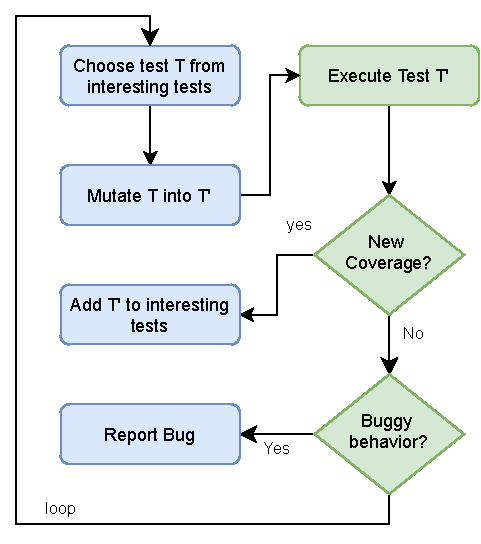
\includegraphics[width=0.8\linewidth]{mutation-fuzzing.pdf}
    \caption{Mutation-based fuzzing feedback loop. First start with a test, i.e.\ set of inputs, then mutate the test, execute it and evaluate how it effected the coverage. If the coverage changed, then the test is interesting else it isn't.}
\label{fig:mut-fuzz}
\end{figure}

\ref{fig:mut-fuzz} shows that in mutation-based fuzzing, we start by defining well-formed inputs, a.k.a.\ seeds, and a coverage metric. 
We then mutate the seeds based on coverage feedback from a previous test in order to obtain new coverage results. 
The fuzzing stops once a target coverage percentage is reached.

We can then define a fuzzer with 3 elements:
\begin{itemize}
\item \textbf{Fuzz server}, which interfaces with the program under test (PUT) and resets it after each test.
\item \textbf{Instrumentation pass}, which is where the coverage-related modifications are made to the PUT.
\item \textbf{Fuzz engine}, which handles test mutation and coverage-feedback analysis.
\end{itemize}

\rewrite{Our project plans to use mainly open-source tools, as we believe that only the open-source
movement can lead to tools for agile hardware development and open libraries for IPs
and verification components.

\subsection{Chisel}

Chisel is a hardware construction language embedded in Scala~\cite{chisel:dac2012}.
Chisel allows the user to write hardware generators in Scala, an object-oriented and functional language. For hardware generation and testing, the full Scala language and Scala and Java
libraries are available.

Chisel is solely a hardware \emph{construction} language, and thus all valid Chisel code
maps to synthesizable hardware.
By separating the hardware construction and hardware verification languages,
it becomes impossible to write non-synthesizable hardware and in turn, speeds up the design process.
As Scala and Java's full power is available to the verification engineer,
the verification process is also made more efficient.

\subsection{ChiselTest}

While Chisel ultimately produces Verilog, which can be tested with industry-standard tools and processes, those generally force the user to pick between simple but limited (e.g., Verilog testbenches) or complex but powerful (e.g., UVM testbenches).

ChiselTest~\cite{chisel:tester2}, a nonsynthesizable testing framework for Chisel, instead emphasizes on usability and simplicity while providing ways to scale up complexity.

Fundamentally, ChiselTest is a Scala library that provides access into the simulator through operations like poke (write value into circuit), peek (read value from circuit, into the test framework), and step (advance time).
As such, tests written in ChiselTest are just Scala programs, imperative code that runs one line after the next.
This structure uses the latest programming language developments that have been implemented into Scala and provides a clean and concise interface, unlike approaches that attempt to reinvent the wheel like UVM.

Furthermore, ChiselTest tries to enable testing best practices from software engineering.
Its lightweight syntax encourages writing targeted unit tests by making small tests easy.
Furthermore, a clear and clean test code also enables the test-as-documentation pattern,
demonstrating a module's behavior from a temporal perspective.}

\subsection{ChiselVerify}

The presented library is part of the ChiselVerify project~\cite{verify:chisel:2020, dobis2021opensource}, available
at \url{https://github.com/chiselverify}.

\subsection{Simulators}

\rewrite{While Chisel designs can be simulated with any simulator that accepts Verilog input, there are trade-offs involved in choosing simulators.
Commercial simulators require expensive licenses, while the open-source Verilator has a high time cost for compilation despite being efficient per-cycle.
On the other hand, Treadle\footnote{\url{https://github.com/freechipsproject/treadle}} is a simulator that operates at the level of Chisel's intermediate representation, FIRRTL\footnote{\url{https://github.com/freechipsproject/firrtl}}.
Simulators like Treadle avoid the step of generating Verilog code and compiling from Verilog, which can vastly reduce the setup time for tests and efficiently run suites of many short tests.

Verilator has the benefit of compiling the Verilog code before simulating it. This is much faster compared to event-driven simulators but also limits the capabilities, as it only works on synchronous designs. Verilator claims to be on par or faster than the ``Big 3'' simulators on single thread. However, it also supports multi-threaded simulation, which can greatly improve simulation times for large designs~\cite{verilator}.}


\subsection{Scala}

\rewrite{The test environment and the driving code is written in Scala. Scala, with its
compatibility with Java, has a very rich open-source library ecosystem.
If you need a tool, e.g., an ELF file reader to load a binary, there will be a Java
library available for it.

Furthermore, we can use all the testing libraries that have been developed for
software development. A popular library is ScalaTest.\footnote{\url{https://www.scalatest.org/}}
A Chisel tester can be embedded
in a ScalaTest component, and a simple \code{sbt test} will execute all the tests.}

\todo{Check what ScalaCheck can offer.}


\section{Fuzzing with Chisel}

\todo{This shall become our main section}

\section{First Experiments}
\label{sec:eval}

\martin{Can we make a quick and dirty (dumb) fuzzing with Leros?}

Although this is a work-in-progress report, we have started with an evaluation.

\martin{Hopefully not just the ALU, maybe the whole processor}

We used an ALU with an accumulator from the Leros processor~\cite{leros:arcs2019}
as our device-under-test (DUT).
The example is simple, but has a combinational part and state in a register, being
a non-trivial circuit for testing.







\subsection{The Road Ahead}

\subsection{Constrained Random Program Generation}
\todo{Tjark can talk about his project here and try to tie it to the overall fuzzing project.}

\todo{ScalaCheck}

This work-in-progress paper is a first sketch of the ideas to...


\subsection{Source Access}

The library for this project is available on GitHub:\\ \url{https://github.com/chiselverify}.
We plan also to regularly publish it on Maven.

\todo{Publish it and provide the info here.}


\section{Conclusion}
\label{sec:conclusion}

This work-in-progress paper is a  initial sketch of supporting testing and verification
of digital designs described in Chisel with fuzzing.




\subsection*{Acknowledgment}

\martin{Do we have something here?}


\bibliographystyle{plain}
% Please do not add any references to msbib.bib.
% They get lost when I 'generate' is again (see Makefile)
\bibliography{../chisel-uvm,../msbib}

\end{document}